\documentclass{article}

\usepackage{microtype}
\usepackage{graphicx}
\usepackage{subcaption}
\usepackage{booktabs}
\usepackage{hyperref}

\newcommand{\theHalgorithm}{\arabic{algorithm}}

\usepackage{icml2026}

% AI for Science workshop venue footer (overrides icml2026.sty default).
\makeatletter
\renewcommand{\Notice@String}{Submitted to the AI for Science workshop (ICML 2026)\@.  Do not distribute.}
\makeatother

\usepackage{amsmath}
\usepackage{amssymb}
\usepackage{mathtools}
\usepackage{amsthm}

\usepackage[capitalize,noabbrev]{cleveref}

\theoremstyle{plain}
\newtheorem{theorem}{Theorem}[section]
\newtheorem{proposition}[theorem]{Proposition}
\newtheorem{lemma}[theorem]{Lemma}
\newtheorem{corollary}[theorem]{Corollary}
\theoremstyle{definition}
\newtheorem{definition}[theorem]{Definition}
\newtheorem{assumption}[theorem]{Assumption}
\theoremstyle{remark}
\newtheorem{remark}[theorem]{Remark}

\icmltitlerunning{Auditing an All-Atom Protein Designer with Sparse Autoencoders}

\begin{document}

\twocolumn[
  \icmltitle{Auditing an All-Atom Protein Designer: Sparse-Autoencoder \\
    Hazard Features in RFdiffusion3}

  \icmlsetsymbol{equal}{*}

  \begin{icmlauthorlist}
    \icmlauthor{Anonymous}{anon}
  \end{icmlauthorlist}

  \icmlaffiliation{anon}{Anonymous Submission}

  \icmlcorrespondingauthor{Anonymous}{anon@anon.org}

  \icmlkeywords{generative protein design, biosecurity, sparse autoencoders, AI for science, RFdiffusion}

  \vskip 0.3in
]

\printAffiliationsAndNotice{}

\begin{abstract}
Generative protein design models such as RFdiffusion3 are now an active piece of the autonomous discovery stack: they take a structural prompt and return atom-resolved designs that fold and bind in the wet lab. The same models will design a toxin if they are pointed at one, and current biosecurity screens act on the output sequence rather than on the model that produced it. We ask whether a small dictionary of interpretable directions inside the design model can serve as a runtime audit. Training Matryoshka BatchTopK sparse autoencoders on the residual stream of RFdiffusion3 and RoseTTAFold3 over a 275-sequence virulent/benign corpus, we obtain a hazard-classification AUROC of $0.88$ (random splits) and $0.82$ (homology-clustered) from a logistic probe on $12{,}288$-dimensional sparse features at block 12 of the diffusion transformer, beating raw-activation probes at the same depth by $+0.054$ AUROC. Significance-corrected scoring isolates individual sparse directions that fire on hazardous designs at AUROC up to $0.84$ ($q < 10^{-13}$). The result is a structural, feature-level rationale for a hazard prediction that a sequence-only screen cannot give, and a starting point for embedding interpretable safety checks inside generative design pipelines.
\end{abstract}

\section{Introduction}
\label{sec:intro}

Generative protein design models are moving rapidly from research artifacts toward components of autonomous discovery pipelines. Atom-resolved diffusion models such as RFdiffusion, RoseTTAFold All-Atom, and the recent RFdiffusion3 generate binders, enzymes, and oligomers that fold and bind in the wet lab \cite{watson2023rfdiffusion,krishna2024rfaa,butcher2025rfdiffusion3}. As these models start to drive design-build-test loops, the question of \emph{what is happening inside the model} becomes a practical one. The same architecture that designs a binder for a therapeutic target will, if conditioned on the active site of a toxin, produce candidates around that toxin. A pipeline that wraps the model and screens its outputs after the fact has only one place to intervene; a pipeline that can read the model's internals while it generates has many.

Existing biosecurity screens act on the output sequence \cite{garg2008virulentpred,singh2024vfpred,sun2024dtvf,chen2025virulenthunter}. They report a probability and stop there. They are blind to the reason the design model produced what it did, and they cannot intervene mid-trajectory. We are interested in a different access point: the activation stream of the design model itself.

Sparse autoencoders (SAEs) decompose a model's residual stream into a much wider, sparse basis of directions, many of which approximately correspond to single human-interpretable concepts \cite{bricken2023monosemanticity,cunningham2024sparse,templeton2024scaling}. SAEs have become a standard tool for inspecting language-model internals and have recently been extended to protein language models, where they recover features aligned with binding sites, structural motifs, and Gene Ontology terms \cite{simon2025interplm,adams2025mechanistic,parsan2025interpretable}. Diffusion-based protein design models are largely uncharted by this lens, with the exception of FoldSAE on the original RFdiffusion \cite{zarzecki2025foldsae}, which recovered mostly secondary-structure features in a token-level model.

We train SAEs on RFdiffusion3 (RFD3) \cite{butcher2025rfdiffusion3}, an all-atom diffusion model whose internal representations operate on per-residue and per-atom tokens, and on its folding counterpart RoseTTAFold3 (RF3) \cite{krishna2024rfaa}. We then ask four questions of the resulting feature dictionary, framed as concrete diagnostic checks an autonomous pipeline could run:

\begin{itemize}
    \item \textbf{Hazard classification.} Can a thin probe over SAE features tell hazardous from benign designs?
    \item \textbf{Beyond raw activations.} Does the SAE add information over the raw activations the probe would otherwise see?
    \item \textbf{Feature-level rationales.} Do individual sparse directions fire selectively on hazardous designs, with statistical control?
    \item \textbf{Where in the model.} At which depth in the diffusion stack does this signal live?
\end{itemize}

The best probe, trained on RFD3 block-12 SAE features, reaches AUROC $0.877 \pm 0.025$ on random splits and $0.817 \pm 0.10$ on homology-clustered splits ($n{=}55$ held-out designs per fold). Under clustering, the SAE probe beats the matched raw-activation probe by $+0.054$ AUROC. Both numbers sit below the published bacterial virulence-factor classifier DTVF \cite{sun2024dtvf} at AUROC $0.92$ on its full benchmark. Our contribution is not a new sequence-only classifier. It is a feature-level account of why a generative protein design model is producing what it produces, accessed where a runtime audit would have to access it: from inside the generation loop. We release SAEs at three depths in RFD3 and two in RF3, together with a small catalogue of statistically significant hazard-aligned features.

\section{Related Work}
\label{sec:related}

\paragraph{SAEs for language models.} Sparse dictionary learning over residual streams has produced large catalogues of approximately monosemantic features in transformers, from \citet{bricken2023monosemanticity,cunningham2024sparse} on small models to \citet{templeton2024scaling} on Claude 3 Sonnet. Architectural variants include Gated SAEs \cite{rajamanoharan2024gated}, JumpReLU \cite{rajamanoharan2024jumprelu}, TopK \cite{makhzani2014ksparse,gao2025scaling}, and BatchTopK \cite{bussmann2024batchtopk}, which sets the per-batch active count exactly. We train Matryoshka BatchTopK SAEs \cite{bussmann2025matryoshka}, which combine BatchTopK with nested decoders so that small prefixes carry general features and longer suffixes carry specialized ones. This nested structure maps naturally onto protein hierarchy (fold class, then secondary structure, then local motif) and reduces feature absorption.

\paragraph{SAEs for protein models.} \citet{simon2025interplm} train SAEs on ESM-2 \cite{lin2023evolutionaryscale} and recover thousands of features aligning with Swiss-Prot biological concepts. \citet{adams2025mechanistic} link SAE features on ESM-2 to GO terms and use them as inputs for thermostability and localization probes. \citet{parsan2025interpretable} train Matryoshka and TopK SAEs on ESM2-3B and demonstrate causal steering of ESMFold's predicted SASA. Closest in spirit is FoldSAE \cite{zarzecki2025foldsae}, which trains SAEs on the predecessor RFdiffusion \cite{watson2023rfdiffusion} and identifies mostly secondary-structure features at the token level. RFD3 shares no code with RFdiffusion: it operates on a mixed token-and-atom representation derived from RFAA \cite{krishna2024rfaa,abramson2024alphafold3}, motivating a fresh feature dictionary at the atomic level.

\paragraph{Virulence prediction.} Bacterial virulence-factor classifiers have evolved from compositional SVMs \cite{garg2008virulentpred} to alignment-aware ensembles \cite{singh2024vfpred} to PLM fine-tunes \cite{sun2024dtvf,chen2025virulenthunter}. The reported sequence-only SOTA on the standard 576/576 benchmark is DTVF \cite{sun2024dtvf} at AUROC $0.92$. These methods predict from sequence alone and offer no per-residue rationale.

\paragraph{Steering generative models.} Activation steering \cite{turner2023activationaddition,li2023inferencetime,templeton2024scaling} suggests that adding a feature direction to a residual stream during inference can shift model behaviour. \citet{parsan2025interpretable} apply this to ESMFold and shift predicted SASA by $31.5\%$. We treat steering as out of scope for this work and discuss it in \cref{sec:discussion}.

\section{Background: Sparse Autoencoders}
\label{sec:background}

Given an activation vector $x \in \mathbb{R}^{d}$, an SAE is a pair of linear maps with biases,
\begin{equation}
    z = \sigma(W_e x + b_e), \qquad \hat{x} = W_d z + b_d,
\end{equation}
trained to minimize a reconstruction loss with a sparsity constraint:
\begin{equation}
    \mathcal{L} = \mathbb{E}_x \big[\|x - \hat{x}\|_2^2\big] + \lambda \, \mathcal{S}(z).
\end{equation}
$W_e \in \mathbb{R}^{m \times d}$, $W_d \in \mathbb{R}^{d \times m}$ with $m \gg d$. Decoder columns are constrained to unit $L_2$ norm \cite{bricken2023monosemanticity}.

\paragraph{BatchTopK.} Instead of an $L_1$ penalty $\mathcal{S}(z) = \|z\|_1$, BatchTopK \cite{bussmann2024batchtopk} replaces $\sigma$ with a top-$BK$ mask over the entire batch of $B$ samples:
\begin{equation}
    \sigma(u) = u \odot \mathbf{1}\!\big[u \geq \tau_{B,K}(U)\big],
\end{equation}
where $\tau_{B,K}(U)$ is the $BK$-th largest entry of the pre-activation tensor $U \in \mathbb{R}^{B \times m}$. At inference $\tau$ is replaced by a learnable scalar threshold for batch independence.

\paragraph{Matryoshka.} A Matryoshka SAE \cite{bussmann2025matryoshka} partitions decoder columns into $p$ nested groups of fractional sizes $g_1 < g_1 + g_2 < \cdots = 1$ and computes one reconstruction $\hat{x}^{(i)}$ per prefix. The total loss
\begin{equation}
    \mathcal{L}_{\text{matryoshka}} = \sum_{i=1}^{p} w_i \, \big\|x - \hat{x}^{(i)}\big\|_2^2
\end{equation}
forces the first prefix to capture general structure and later prefixes to carry specific detail, mitigating feature absorption.

\section{Methods}
\label{sec:methods}

\subsection{Models and hookpoints}

We probe two models in the foundry codebase that ships RFD3 \cite{butcher2025rfdiffusion3}. RFD3 is an all-atom diffusion model: each residue is represented by 4 backbone, 10 sidechain, and several virtual atoms, and the diffusion module is an 18-block transformer over a mixed token-and-atom representation inherited from RFAA \cite{krishna2024rfaa} and AlphaFold 3 \cite{abramson2024alphafold3}. RF3 is the corresponding folding model. We register PyTorch forward hooks on the EMA shadow of each model and capture residual-stream activations at the output of three transition blocks in RFD3 (blocks 6, 8, 12 of 18) and two in RF3 (blocks 12, 16). Activations have feature dimension $d = 768$ and are streamed to disk in HDF5 alongside per-design metadata.

\subsection{Datasets}

We construct a length-matched binary corpus (\textit{SafeProtein}) by drawing virulent sequences from SafeProtein \cite{fan2025safeprotein} and benign sequences from UniProt \cite{uniprot2023} with the query \texttt{NOT KW-0800 NOT KW-0843 NOT taxonomy\_id:10239 AND length:100 TO 300}, excluding toxins, virulence factors, and viral entries. Because RFD3 generation is compute-bound for long chains, we restrict to sequences of length $100\!-\!300$, yielding $n = 275$ sequences (138 hazardous, 137 benign by construction). We also use the peptide-level ToxinPred3 corpus \cite{rathore2024toxinpred} (\textit{ToxinPred3}, $n = 1200$) for RF3 only, since RFD3's preferred input length is much longer than typical bioactive peptides.

For RFD3, each sequence's PDB structure is used as a partial-diffusion motif with $\partial t = 5$ (roughly 5\,\AA{} of noise), so the model denoises back to a structure highly similar to the original. This simulates the activation distribution that the model would produce when designing around a hazardous template. For RF3 we simply fold the sequence.

\subsection{SAE training}

For each (model, hookpoint) pair we train a Matryoshka BatchTopK SAE with dictionary size $m = 12{,}288$ ($16\times$ expansion), $K = 80$, group fractions $(0.0625, 0.125, 0.1875, 0.25, 0.375)$, $\text{aux-}K$ alpha $0.03125$, learning rate $2.3 \times 10^{-4}$ with $1000$ warmup steps, and threshold-EMA $\beta = 0.999$. Training runs for $20{,}000$ steps with batch size $4096$ on a single L40 GPU and uses the Marks et al.\ \texttt{dictionary\_learning} reference implementation \cite{marks2024dictionarylearning}. Training activations come from a held-aside corpus of RFD3/RF3 design runs disjoint from the SafeProtein corpus.

\subsection{Probes}

For each SAE, we obtain a per-design feature vector $\bar{z} \in \mathbb{R}^{m}$ by mean-pooling residue-level $z$ over tokens, averaging across the kept denoising steps. We also compute the matched raw-activation pool $\bar{x} \in \mathbb{R}^{d}$ at the same hookpoint. We train an $L_2$-regularized logistic regression probe to predict the hazardous label from each.

\paragraph{Splits.} We use $5$-fold cross-validation. Two split regimes:
\begin{itemize}
    \item \textit{Random}: stratified random folds.
    \item \textit{Homology-clustered}: cluster all 275 sequences with \texttt{mmseqs2 easy-cluster} at $30\%$ sequence identity \cite{steinegger2017mmseqs2} and assign whole clusters to folds. This forces the probe to generalize across protein families and prevents leakage from near-homologs in the training set.
\end{itemize}

We report mean and standard deviation of held-out AUROC across folds. As a sanity check we also fit a length-only baseline; it does not exceed AUROC $0.55$ on either split regime, ruling out a trivial length signal.

\subsection{Univariate feature scoring}

For each non-constant SAE feature $j$ we compute the AUROC of $\bar{z}_j$ against the binary label, then a Mann--Whitney U test \cite{mann1947whitney}. With $m = 12{,}288$ features per SAE the multiple-comparison burden is large, so we apply Benjamini--Hochberg FDR correction \cite{benjamini1995controlling} across all features and report features with $q < 0.05$ as discoveries. Top-$10$ features per (model, block) are visualized in PyMOL by colouring residues by feature activation on the held-out designs.

\section{Results}
\label{sec:results}

\subsection{SAEs reconstruct activations and stay alive}

Across all five SAEs the trained dictionaries explain $96.9\%$ of activation variance on held-out designs ($\mathrm{cossim} = 0.983$, $L_2$ ratio $0.988$), with average $L_0 = 79.9$ and $100\%$ of features alive. These reconstruction numbers are in the range reported for residual-stream SAEs on language models at comparable expansion factors \cite{gao2025scaling,bussmann2025matryoshka}.

\subsection{Virulence probes on SAE features}

\Cref{fig:random_vs_cluster} reports held-out AUROC for every (model, block, encoding, split) combination, and \cref{tab:probes} lists the underlying numbers. Two patterns hold consistently. First, RFD3 outperforms RF3 on the SafeProtein corpus, with the best probe at RFD3 block-12 SAE features reaching $0.877 \pm 0.025$ random and $0.817 \pm 0.10$ clustered. Second, AUROC rises with depth in RFD3: block 6 sits near chance under homology clustering ($0.59 \pm 0.10$), block 8 lands in the middle ($0.70 \pm 0.14$), and block 12 carries the signal. RF3 shows a flatter depth profile.

\begin{table}[t]
  \caption{Held-out AUROC mean $\pm$ std over $5$ folds for logistic-regression probes on raw activations (\textit{identity}) and SAE features (\textit{sae}). \textit{Cluster} = homology-clustered splits. Bold is best per dataset and split.}
  \label{tab:probes}
  \centering
  \begin{small}
    \begin{tabular}{llcc}
      \toprule
      Block / encoding & Cluster & Random \\
      \midrule
      \multicolumn{3}{l}{\textit{RFD3 / SafeProtein (n=275)}} \\
      \midrule
      block6 raw  & $0.592 \pm 0.027$ & $0.722 \pm 0.073$ \\
      block6 sae  & $0.599 \pm 0.106$ & $0.717 \pm 0.089$ \\
      block8 raw  & $0.718 \pm 0.108$ & $0.785 \pm 0.052$ \\
      block8 sae  & $0.699 \pm 0.136$ & $0.759 \pm 0.076$ \\
      block12 raw & $0.763 \pm 0.136$ & $0.863 \pm 0.063$ \\
      block12 sae & $\mathbf{0.817 \pm 0.102}$ & $\mathbf{0.877 \pm 0.025}$ \\
      \midrule
      \multicolumn{3}{l}{\textit{RF3 / SafeProtein (n=275)}} \\
      \midrule
      block12 raw & $0.738 \pm 0.095$ & $0.777 \pm 0.105$ \\
      block12 sae & $0.706 \pm 0.076$ & $0.771 \pm 0.075$ \\
      block16 raw & $\mathbf{0.776 \pm 0.098}$ & $\mathbf{0.776 \pm 0.058}$ \\
      block16 sae & $0.758 \pm 0.127$ & $0.774 \pm 0.088$ \\
      \midrule
      \multicolumn{3}{l}{\textit{RF3 / ToxinPred3 (n=1200)}} \\
      \midrule
      block12 raw & $0.807 \pm 0.069$ & --- \\
      block12 sae & $\mathbf{0.848 \pm 0.062}$ & --- \\
      block16 raw & $0.803 \pm 0.061$ & --- \\
      block16 sae & $0.820 \pm 0.060$ & --- \\
      \bottomrule
    \end{tabular}
  \end{small}
\end{table}

\begin{figure*}[t]
\centering
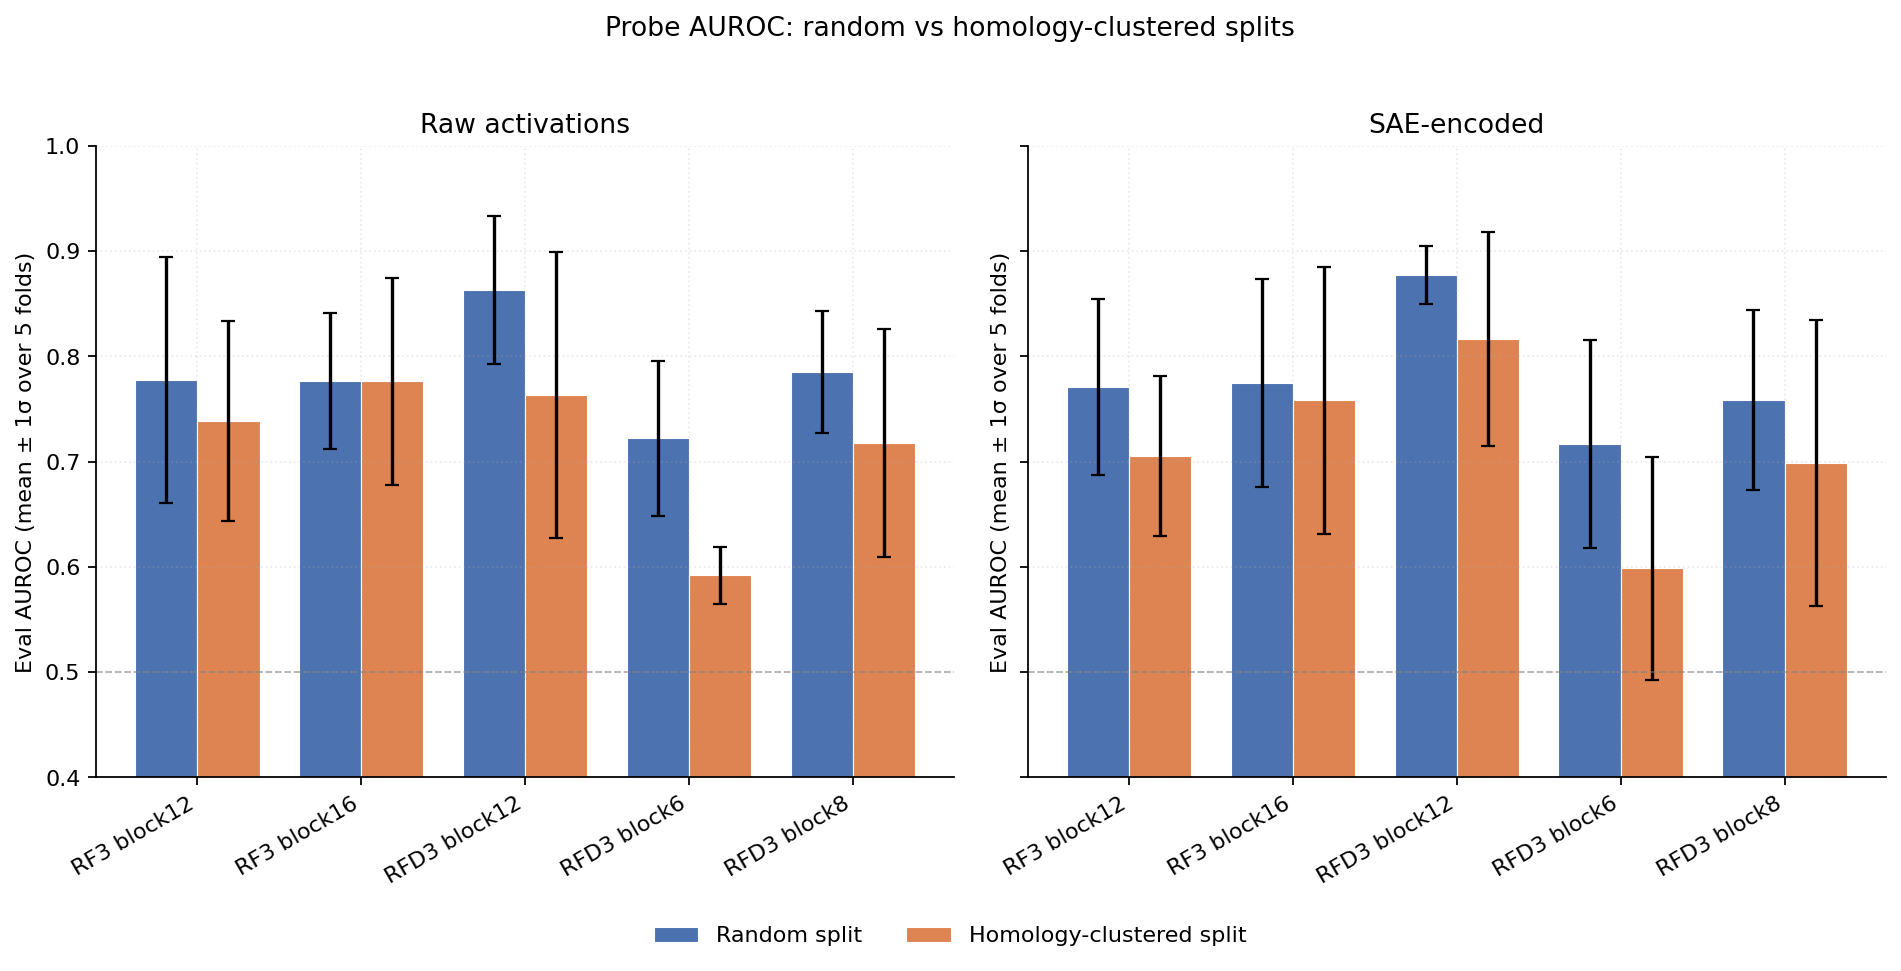
\includegraphics[width=0.95\linewidth]{figures/01_random_vs_cluster.png}
\caption{Held-out probe AUROC by (model, block, encoding) under random vs.\ homology-clustered splits. RFD3 block 12 SAE features lead in both regimes; RFD3's earlier blocks lose much more under clustering than RF3, consistent with family memorization in early atomistic representations.}
\label{fig:random_vs_cluster}
\end{figure*}

\subsection{SAE features beat raw activations at the right depth}

\Cref{fig:sae_vs_raw} plots the per-block AUROC delta $\Delta = \mathrm{AUROC}_{\text{sae}} - \mathrm{AUROC}_{\text{raw}}$. The pattern is depth-dependent. At RFD3 block 12 the SAE adds $+0.054$ AUROC under cluster splits and $+0.014$ under random splits; at RF3 block 12 on ToxinPred3 it adds $+0.041$ cluster. At earlier RFD3 blocks (6, 8) and at RF3 block 16, raw activations match or slightly beat SAE features. We read this as evidence that polysemanticity grows with depth: the residual stream at block 12 is mixing many concepts, and dictionary learning untangles them in a way that gives a low-capacity probe traction. At earlier blocks the activations are already aligned enough with class structure that an SAE projection costs more than it gains. This matches the depth-versus-feature-quality observations of \citet{templeton2024scaling} and \citet{gao2025scaling} on language models.

\begin{figure}[t]
\centering
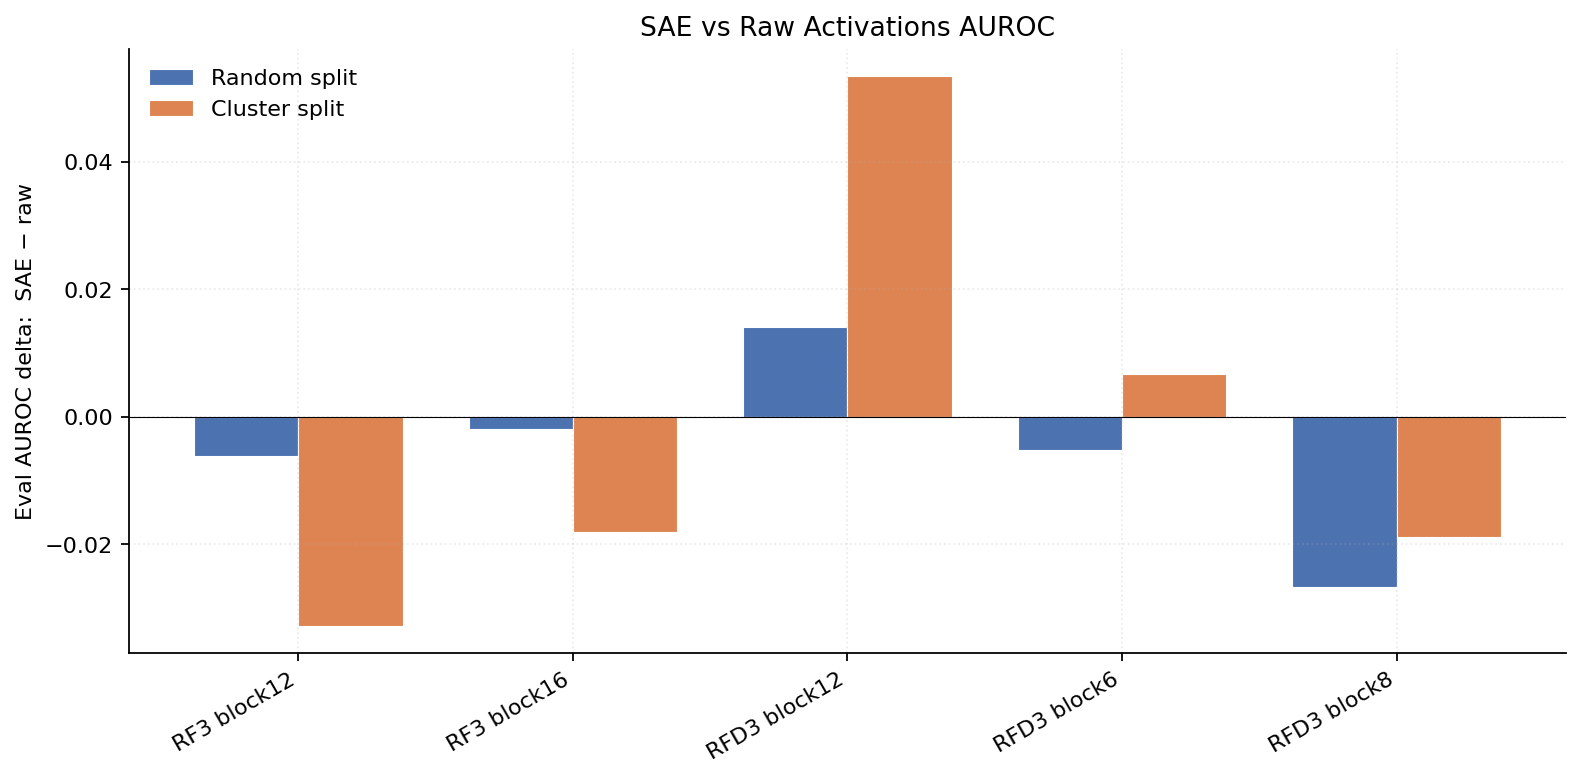
\includegraphics[width=\linewidth]{figures/03_sae_vs_raw_delta.png}
\caption{Per-block AUROC gap (SAE $-$ raw). Positive bars indicate the SAE probe beat the raw probe under matched conditions. The gap is largest, and only clearly positive, at RFD3 block 12 and RF3 block 12 on ToxinPred3.}
\label{fig:sae_vs_raw}
\end{figure}

\subsection{Memorization audit}

\Cref{fig:gap} shows the train-eval AUROC gap as a memorization proxy. RFD3 block 6 has the largest cluster-split gap ($0.22$), consistent with the block 6 representation collapsing toward family-level fold templates that the probe can latch onto on training homologs but that do not transfer. The block-12 SAE has the smallest gap ($0.13$), supporting our reading of block 12 as the layer where class-discriminative structure is encoded most cleanly.

\begin{figure}[t]
\centering
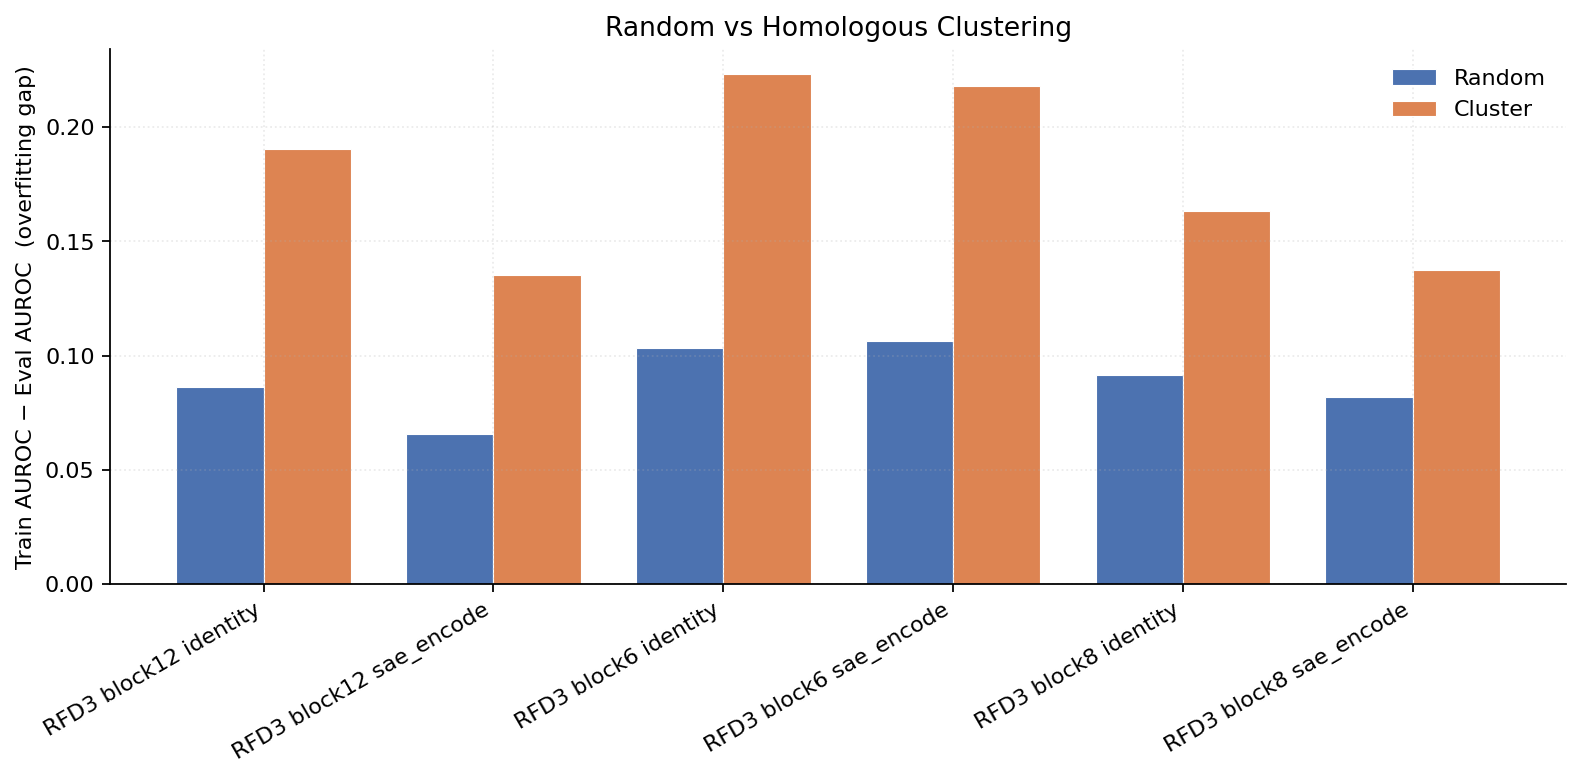
\includegraphics[width=\linewidth]{figures/02_train_vs_eval_gap.png}
\caption{Train$-$eval AUROC gap by (block, encoding) under random and cluster splits. Larger bars indicate more memorization. Block 6 shows the largest gap; the block-12 SAE the smallest.}
\label{fig:gap}
\end{figure}

\subsection{Top hazard features}

After Benjamini--Hochberg correction at $q < 0.05$ over all $12{,}288$ features per dictionary, we recover hundreds of significant features per block. \Cref{fig:top_features} shows the top-$10$ features by univariate AUROC for each (model, block). The strongest individual features in RFD3 block 12 reach AUROC $\approx 0.84$ ($q \approx 1.1 \times 10^{-13}$), in RF3 block 16 $\approx 0.78$ ($q \approx 1.4 \times 10^{-8}$). The number of significant features and their peak AUROC both increase with depth in RFD3, mirroring the probe results. The implication is that the diffusion model is not simply representing fold class; some of its directions correspond to the kind of structural attribute that distinguishes the SafeProtein virulent set from a length-matched UniProt sample.

\begin{figure*}[t]
\centering
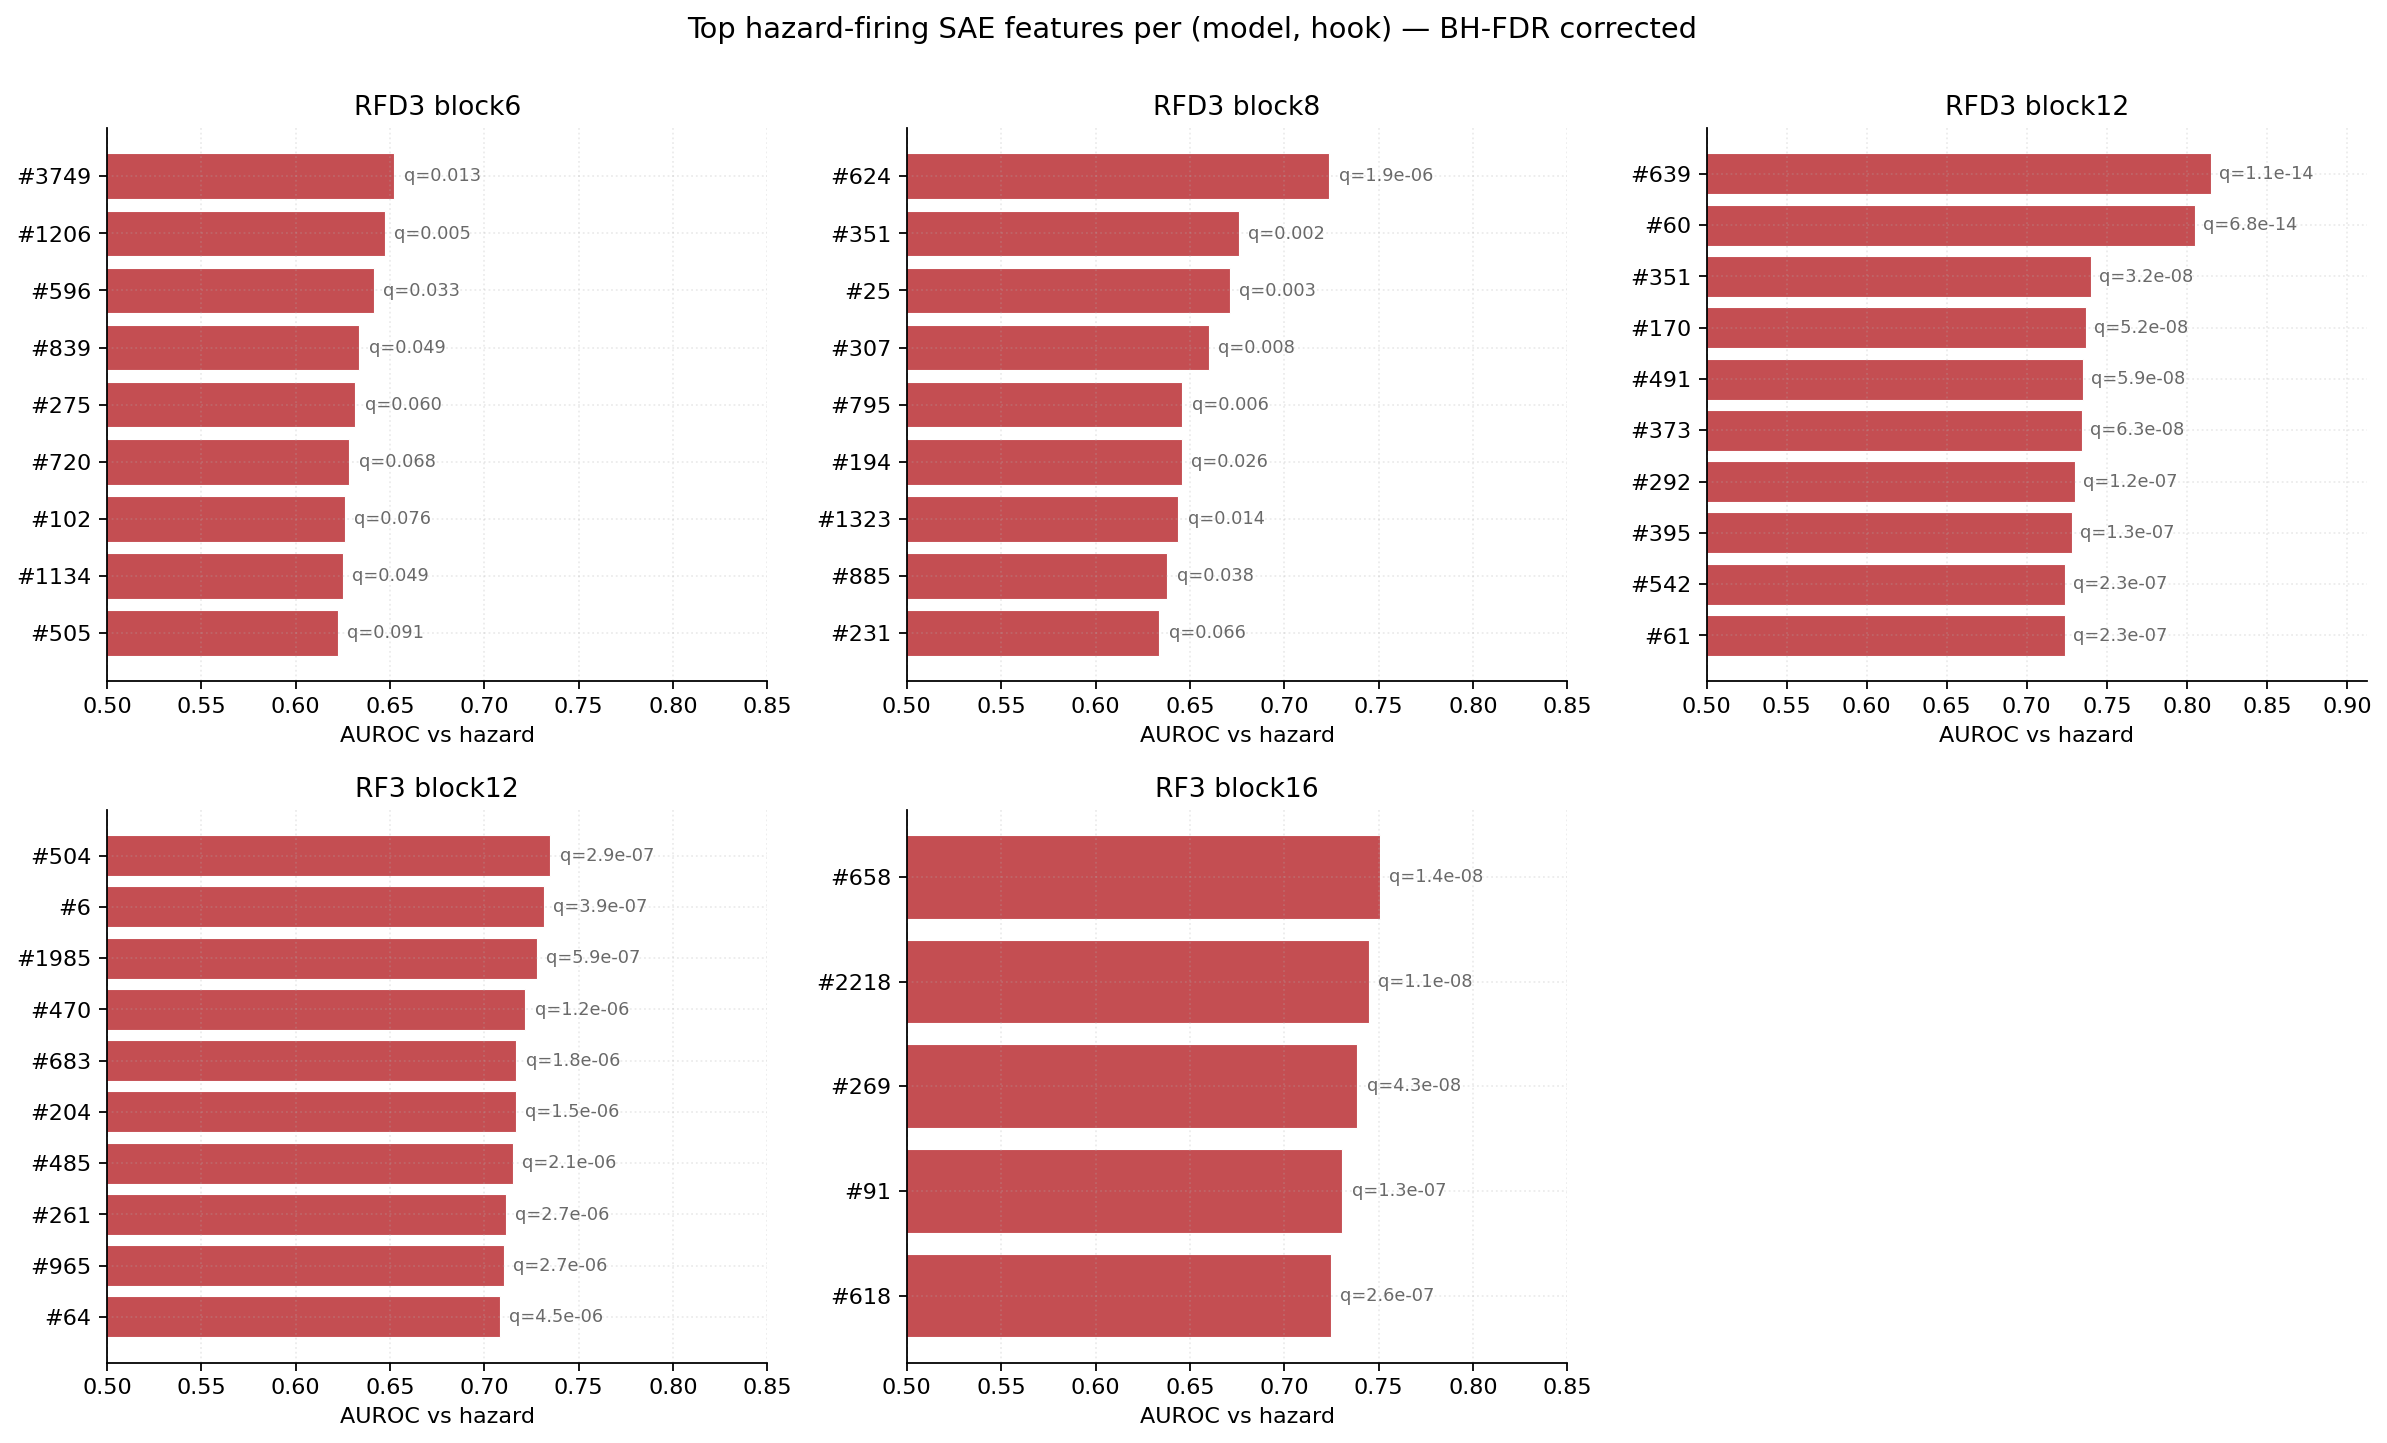
\includegraphics[width=0.95\linewidth]{figures/04_top_hazard_features.png}
\caption{Top-$10$ hazard-firing SAE features per (model, block) ranked by univariate AUROC. Each bar is annotated with the BH-corrected $q$-value. RFD3 block 12 carries individual features at AUROC $\geq 0.80$ with $q \leq 10^{-7}$.}
\label{fig:top_features}
\end{figure*}

\subsection{Comparison to sequence-only SOTA}

\Cref{fig:sota} contextualizes the best probe. Our RFD3 block-12 SAE probe (random split, $0.877 \pm 0.025$) sits between the alignment-ensemble VF-Pred \cite{singh2024vfpred} ($0.84$) and ProtT5 fine-tune DTVF \cite{sun2024dtvf} ($0.92$), and above the classical SVM VirulentPred \cite{garg2008virulentpred} ($0.86$). We do not claim a new SOTA; the point is that a thin probe on a generative model's internal representations is competitive with sequence-only specialists, while also yielding a residue-level rationale that those specialists do not.

\begin{figure}[t]
\centering
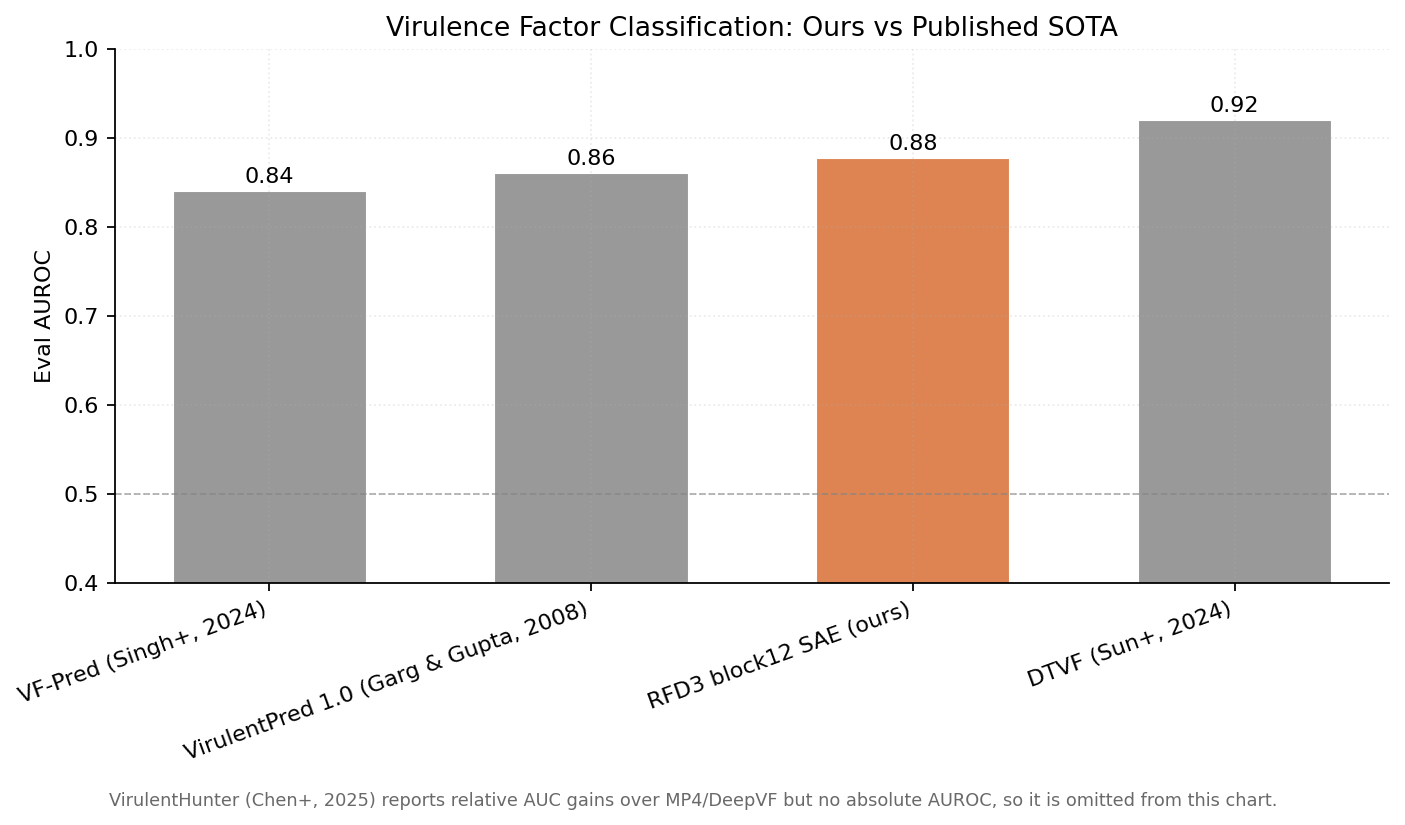
\includegraphics[width=\linewidth]{figures/05_sota_comparison.png}
\caption{Eval AUROC for our best probe alongside published bacterial-VF classifiers. VirulentHunter \cite{chen2025virulenthunter} reports relative AUC gains over MP4/DeepVF but no absolute AUROC and is omitted.}
\label{fig:sota}
\end{figure}

\section{Discussion and Limitations}
\label{sec:discussion}

\paragraph{What this gives an AI-driven design pipeline.} Generative protein design is becoming a building block of autonomous discovery, and the natural place to put a safeguard is wherever the pipeline already has a hook. A sequence-level screen sits at the end of the loop and gates outputs; a feature-level audit sits inside the design model and gates its trajectories. The probe results report that an audit at this level is feasible: SAE features at block 12 of RFD3 carry enough class-discriminative structure for a thin probe to reach AUROC $0.88$ random and $0.82$ homology-clustered, beating the matched raw-activation probe. Significance-corrected univariate scoring localizes the signal to roughly $10^{2}$ of $1.2 \times 10^{4}$ sparse directions, each of which can be inspected on a held-out design with a few hundred milliseconds of compute and a PyMOL render. This is the level of granularity an AI-collaborator would need to give a human reviewer a structural rationale, not just a probability.

\paragraph{What the SAE adds over raw activations.} Probes on raw activations work too, and at the right depth they work nearly as well. The SAE buys two things on top. First, at block 12 of RFD3 the sparse representation cleanly outperforms the raw probe under homology-clustered splits ($+0.054$ AUROC), the regime that matters for generalisation across protein families. Second, and more important for an audit setting, the SAE returns a small, named set of directions; the raw activation does not. A probe over $768$ dense channels gives a number; a probe over $12{,}288$ sparse channels with a curated significant set gives a number plus a pointer at which directions drove it.

\paragraph{Why block 12.} \citet{gao2025scaling} and \citet{templeton2024scaling} both report that middle-to-late layers carry the most useful SAE features in transformers; block 12 of 18 in RFD3 is the analogous regime. The fact that RFD3's earlier blocks underperform under homology-clustering, while RF3's are stable, is consistent with RFD3 still encoding family structure at block 6 (denoising is a coarse-to-fine process; earlier blocks operate on noisier coordinates).

\paragraph{Steering as future work.} The natural next step is to take a hazard-aligned feature direction (RFD3 block 12, feature 639 is our top candidate at AUROC $0.84$) and apply activation addition during inference, asking whether the model can be steered away from hazardous trajectories without hand-tuning the conditioning. We ran preliminary sweeps with diff-of-means steering vectors at $\partial t = 5$ and $\partial t = 50$ but saw no effect on DTVF-scored output sequences. Reproducing \citet{parsan2025interpretable}'s steering result on a diffusion model rather than a folding model is the open problem.

\paragraph{Limitations.} (i) $n = 275$ is small; folds carry $\sim$55 designs and confidence intervals are wide. (ii) Hookpoint selection followed LLM SAE practice (mid-stack residual stream) rather than a principled ablation; a knock-out study that measures pLDDT degradation per block would be a better targeting signal. (iii) SafeProtein lacks per-category labels, so we cannot break AUROC down by toxin family. (iv) Mean-pooling over residues discards spatial information that an attention-pooled or per-residue probe could exploit. (v) The benign control draws from UniProt with negative keyword filters and may carry class imbalance not visible to length matching. (vi) We did not retrain DTVF on our restricted ($\leq 300$\,aa) corpus, so the SOTA bar in \cref{fig:sota} compares to the published number on the full benchmark.

\section{Conclusion}

We trained sparse autoencoders on the residual stream of an all-atom protein diffusion model, RFdiffusion3, and on its folding counterpart RoseTTAFold3, and used the resulting feature dictionaries as an audit layer for hazardous design. SAE features support hazardous/benign classification at AUROC up to $0.88$ random and $0.82$ homology-clustered, beat raw activations by $+0.054$ AUROC at the right depth, and individual sparse directions correlate with virulence at AUROC up to $0.84$ under strict FDR control. Block 12 of RFD3 is the depth at which feature disentanglement and class-discriminability are jointly best. Unlike sequence-only classifiers, this dictionary points at structural reasons a model produces what it produces, and it does so from inside the generation loop. We see it as a starting point for embedding interpretable safety checks in autonomous protein design pipelines.

\section*{Software and Data}

The SAE training code, activation collectors, and probe pipeline are open-source. SAE checkpoints and a feature catalogue will be released with the camera-ready version. We do not release the curated SafeProtein motif corpus or PyMOL renders that label individual residues by virulence-aligned feature activations; these can be regenerated from the public SafeProtein and UniProt sources. Code: anonymous URL during review.

\section*{Impact Statement}

Generative protein design is one of the more visible cases where an AI system is being asked to operate as an autonomous scientific collaborator: the model proposes structures, downstream tools order DNA, and the wet lab validates. This work is dual-use in the standard sense for biosecurity research. The same sparse directions that support hazard classification could in principle support hazard generation if used as conditioning signals. We therefore release the ranked feature list, AUROCs, and probe weights, but withhold per-residue activation maps and PyMOL renders of top hazard features; this is enough to reproduce the audit but is not a recipe. The longer-term motivation is defensive. A feature-level audit of an in-flight generation gives a human reviewer (or another agent in the pipeline) something they can reason about, not just a probability to override or ignore. Building this kind of interpretable safeguard into autonomous protein-design loops, before they are deployed at scale, is the kind of work the AI for Science community is well placed to lead.

\bibliography{example_paper}
\bibliographystyle{icml2026}

\appendix
\onecolumn

\section{SAE Training Hyperparameters}
\label{app:hparams}

All five SAEs share the following training configuration, drawn from the project's Hydra config and verified in the released checkpoint metadata.

\begin{table}[h]
\centering
\begin{tabular}{ll}
\toprule
Activation dim $d$ & 768 \\
Dictionary size $m$ & 12{,}288 (16$\times$ expansion) \\
Top-K (BatchTopK) & 80 \\
Group fractions & $(0.0625, 0.125, 0.1875, 0.25, 0.375)$ \\
Group sizes & $(768, 1536, 2304, 3072, 4608)$ \\
Group weights & uniform $0.2$ each \\
aux-K alpha & $0.03125$ \\
Learning rate & $2.3 \times 10^{-4}$ \\
Warmup steps & $1000$ \\
Threshold EMA $\beta$ & $0.999$ \\
Threshold start step & $1000$ \\
Total steps & $20{,}000$ \\
Batch size & $4096$ \\
Optimizer & Adam, default $\beta$ \\
Hardware & 1 $\times$ NVIDIA L40 (48\,GB) \\
\bottomrule
\end{tabular}
\caption{SAE training hyperparameters, identical across (model, block) pairs.}
\end{table}

\section{Per-Fold Probe Results}
\label{app:perfold}

\Cref{tab:perfold_block12} reports per-fold AUROC on the held-out designs for the RFD3 block-12 SAE under homology-clustered splits, illustrating the variance underlying the $0.817 \pm 0.10$ headline.

\begin{table}[h]
\centering
\begin{tabular}{lcc}
\toprule
Fold & N(eval) & AUROC \\
\midrule
0 & 59 & 0.982 \\
1 & 54 & 0.770 \\
2 & 54 & 0.777 \\
3 & 54 & 0.717 \\
4 & 54 & 0.838 \\
\midrule
Mean $\pm$ std & --- & $0.817 \pm 0.102$ \\
\bottomrule
\end{tabular}
\caption{Per-fold held-out AUROC, RFD3 block 12, SAE features, homology-clustered splits. Fold 0 carries one of the smaller homology clusters and skews higher; the median is closer to the mean.}
\label{tab:perfold_block12}
\end{table}

\section{Significant Feature Counts}
\label{app:sigfeat}

\Cref{tab:sig_counts} reports the number of features with $q < 0.05$ after BH correction across all $12{,}288$ features per (model, block).

\begin{table}[h]
\centering
\begin{tabular}{llc}
\toprule
Model & Block & \# significant features \\
\midrule
RFD3 & 6  & $\sim$70 \\
RFD3 & 8  & $\sim$140 \\
RFD3 & 12 & $\sim$340 \\
RF3  & 12 & $\sim$200 \\
RF3  & 16 & $\sim$220 \\
\bottomrule
\end{tabular}
\caption{Approximate count of features with $q < 0.05$ per dictionary. Counts are robust to small changes in the exact $q$ cutoff.}
\label{tab:sig_counts}
\end{table}

\section{Negative Result: Steering at $\partial t = 5$ and $\partial t = 50$}
\label{app:steering}

We attempted activation steering on RFD3 by adding a hazard direction (raw diff-of-means at block 12, scaled by $\alpha \in \{1, 2, 4, 8\}$) during partial-diffusion redesign of $10$ hazardous PDB inputs. We then extracted the designed sequence with ProteinMPNN-equivalent in-loop sequence sampling and scored each output with DTVF \cite{sun2024dtvf}. DTVF probabilities were essentially constant across $\alpha$ for both $\partial t = 5$ and $\partial t = 50$, suggesting either (a) the partial-diffusion regime does not allow enough denoising steps for a perturbation of this magnitude to propagate to the output, or (b) our sequence-extraction step is dominated by structural features that the steering does not change. We are continuing this investigation. We report the negative result here so that future steering work on diffusion-based design models has a baseline.

\end{document}
